%!TEX root = ../main.tex
\section{Data}
\label{sec:data}
In the data section, we describe the source of our data and how the factor strategies are constructed. We then present summary statistics including tests for autocorrelation and volatility clustering, as well as quantile-quantile (QQ) plots. Finally, we discuss the unconditional correlation of the factor strategies.

\subsection{Data description}

Factor return series are downloaded from Ken French's data library.\footnote{Ken French Data Library. (2016). \textit{Fama/French 5 Factors (2x3) [Daily]} and \textit{Momentum Factor (Mom) [Daily]}. Available from: \url{http://mba.tuck.dartmouth.edu/pages/faculty/ken.french/data_library.html}} We download the daily Fama-French five-factor data set and merge this with the daily momentum data set. Both are available since 1963-07-01, making 1963-07-05 the first week of data. In our sample, 2016-07-01 is the last data point. While the related papers \textcite{FF2015} and \textcite{Asness2015} both use monthly data, we choose the weekly frequency for two main reasons: (1) We take a portfolio perspective rather than an asset pricing perspective, and believe that a more frequent horizon than monthly data is relevant for both rebalancing and risk management objectives, and (2) Due to computational limitations, the copula methodology discourages from going to the daily frequency as optimizations become significantly more time-consuming.

We proceed with descriptions of how factors are constructed. The Mkt-RF factor is long the value-weighted return of CRSP firms on NYSE, AMEX or NASDAQ with CRSP share codes 10 or 11 and short the one-month Treasury bill rate. The remaining return series are based on zero-cost portfolios that are long certain equities and short other equities, according to a 2 x 3 sort: First, firms are sorted into one of two size groups, small and big, depending on whether the market cap is above or below the median. In the small and big firm groups, each factor then sorts into one of three groups depending on whether the variable of interest falls below the 30\textsuperscript{th} percentile, between the 30\textsuperscript{th} and the 70\textsuperscript{th} or above the 70\textsuperscript{th}. For the five-factor data set, the factors are:
\begin{itemize}
  \item High-minus-low, is long firms above the 70\textsuperscript{th} percentile B/M (high) and short stocks below the 30\textsuperscript{th} percentile, in the small and big firm group respectively.
  \item Robust-minus-weak, is long firms above the 70\textsuperscript{th} percentile operating profitability and short firms below the 30\textsuperscript{th} percentile. 
  \item Conservative-minus-aggressive, is long firms above the 70\textsuperscript{th} percentile total asset growth and short firms below the 30\textsuperscript{th} percentile. 
  \item Small-minus-big, is long firms below the 50\textsuperscript{th} percentile market cap and short firms above the 50\textsuperscript{th} percentile, in each of the three groups HML, RMW and CMA.
  \item Momentum, is long firms above the 70\textsuperscript{th} percentile prior 2-12 month return (i.e. excluding the last month) and short stocks below the 30\textsuperscript{th} percentile, in the small and big firm group respectively.
\end{itemize}
The sort ensures that SMB includes firms small and big firms equally from the other factors, and that the other factors include equal amounts of small and big firms, as noted in the equations below. Note that momentum originates from a different data set and does not affect the SMB compisition.
\begin{align*}
  \text{HML} &= 1/2 \cdot (\text{Small value} + \text{Big value}) - 1/2 \cdot (\text{Small growth} + \text{Big growth}) \\
  \text{RMW} &= 1/2 \cdot (\text{Small robust} + \text{Big robust}) - 1/2 \cdot (\text{Small weak} + \text{Big weak}) \\
  \text{CMA} &= 1/2 \cdot (\text{Small conservative} + \text{Big conservative}) - 1/2 \cdot (\text{Small aggressive} + \text{Big aggressive}) \\
  \text{SMB} &= 1/3 \cdot (\text{SMB}_\text{HML} + \text{SMB}_\text{RMW} + \text{SMB}_\text{CMA}) \\
  \text{Mom} &= 1/2 \cdot (\text{Small high} + \text{Big high}) - 1/2 \cdot (\text{Small low} + \text{Big low})
\end{align*}

French's financial statement data originates from Compustat, stock return data from CRSP and Treasury return data from Ibbotson Associates.

\subsection{Summary statistics}
% Table created by stargazer v.5.2 by Marek Hlavac, Harvard University. E-mail: hlavac at fas.harvard.edu
% Date and time: lör, okt 15, 2016 - 22:22:53
\begin{table}[!htbpp] \centering 
  \scriptsize
  \renewcommand{\arraystretch}{1.2}
  \caption{Summary statistics of weekly returns on factor strategies. \\ \quad \\
  Kurtosis is excess kurtosis, i.e. zero for a normal distribution. LB [5/10] is the weighted Ljung-Box test up to 5/10 lags of \textcite{FisherGallagher2012}, where the null hypothesis is no autocorrelation.}
  \label{tab:summarydata} 
\begin{tabularx}{\textwidth}{@{\extracolsep{5pt}} X r r r r r r} 
  \toprule
  & Mkt.RF & SMB & Mom & HML & CMA & RMW \\ 
\midrule
Observations & $2,766$ & $2,766$ & $2,766$ & $2,766$ & $2,766$ & $2,766$ \\ 
Maximum & $0.126$ & $0.060$ & $0.120$ & $0.117$ & $0.054$ & $0.094$ \\ 
Minimum & $$-$0.198$ & $$-$0.098$ & $$-$0.175$ & $$-$0.083$ & $$-$0.044$ & $$-$0.062$ \\ 
Mean & $0.001$ & $0.000$ & $0.001$ & $0.001$ & $0.001$ & $0.001$ \\ 
Median & $0.003$ & $0.001$ & $0.002$ & $0.000$ & $0.000$ & $0.000$ \\ 
Volatility & $0.022$ & $0.012$ & $0.019$ & $0.012$ & $0.009$ & $0.009$ \\
Skewness & $$-$0.688$ & $$-$0.504$ & $$-$1.390$ & $0.331$ & $0.306$ & $0.724$ \\ 
Kurtosis (excess) & $6.191$ & $4.997$ & $11.987$ & $7.318$ & $3.149$ & $13.005$ \\
\midrule
Return LB [5] p-value & $0.263$ & $0.000$ & $0.000$ & $0.000$ & $0.000$ & $0.000$ \\ 
Return LB [10] p-value & $0.007$ & $0.000$ & $0.000$ & $0.000$ & $0.000$ & $0.000$ \\ 
Return\textsuperscript{2} LB [5] p-value & $0.000$ & $0.000$ & $0.000$ & $0.000$ & $0.000$ & $0.000$ \\ 
Return\textsuperscript{2} LB [10] p-value & $0.000$ & $0.000$ & $0.000$ & $0.000$ & $0.000$ & $0.000$ \\ 
\bottomrule
\end{tabularx} 
\end{table}
For all series, there are 2,766 consecutive data points and no missing data. Mkt-RF is the most volatile and extreme of the series, with weekly returns between -19.8\% and 12.6\% and a standard deviation of 2.2\%. Among the value strategies, CMA and RMW seem to be less extreme than HML, with less negative minimums and smaller standard deviations. The factor strategies have excess kurtosis, or fat tails, which is typical for financial returns. The excess kurtoses of the Mom, HML and RMW factors are even higher than the kurtosis of the Mkt-RF factor. However, while market returns are negatively skewed, the value strategies HML, CMA and RMW instead exhibit positive skewness. QQ-plots versus normal theoretical quantiles in \autoref{fig:qq_returns} graphically show the non-normality.
\begin{figure}[htbp]
  \centering
  \footnotesize
  \renewcommand{\arraystretch}{1.2}
  \caption{QQ-plots versus normal distribution \\ \quad \\ 
  Quantile-quantile plots of theoretical (normal) and sample quantiles. Data from a normal distribution should line up on the dashed line. Weekly returns 1963--2016.}
  \label{fig:qq_returns}
  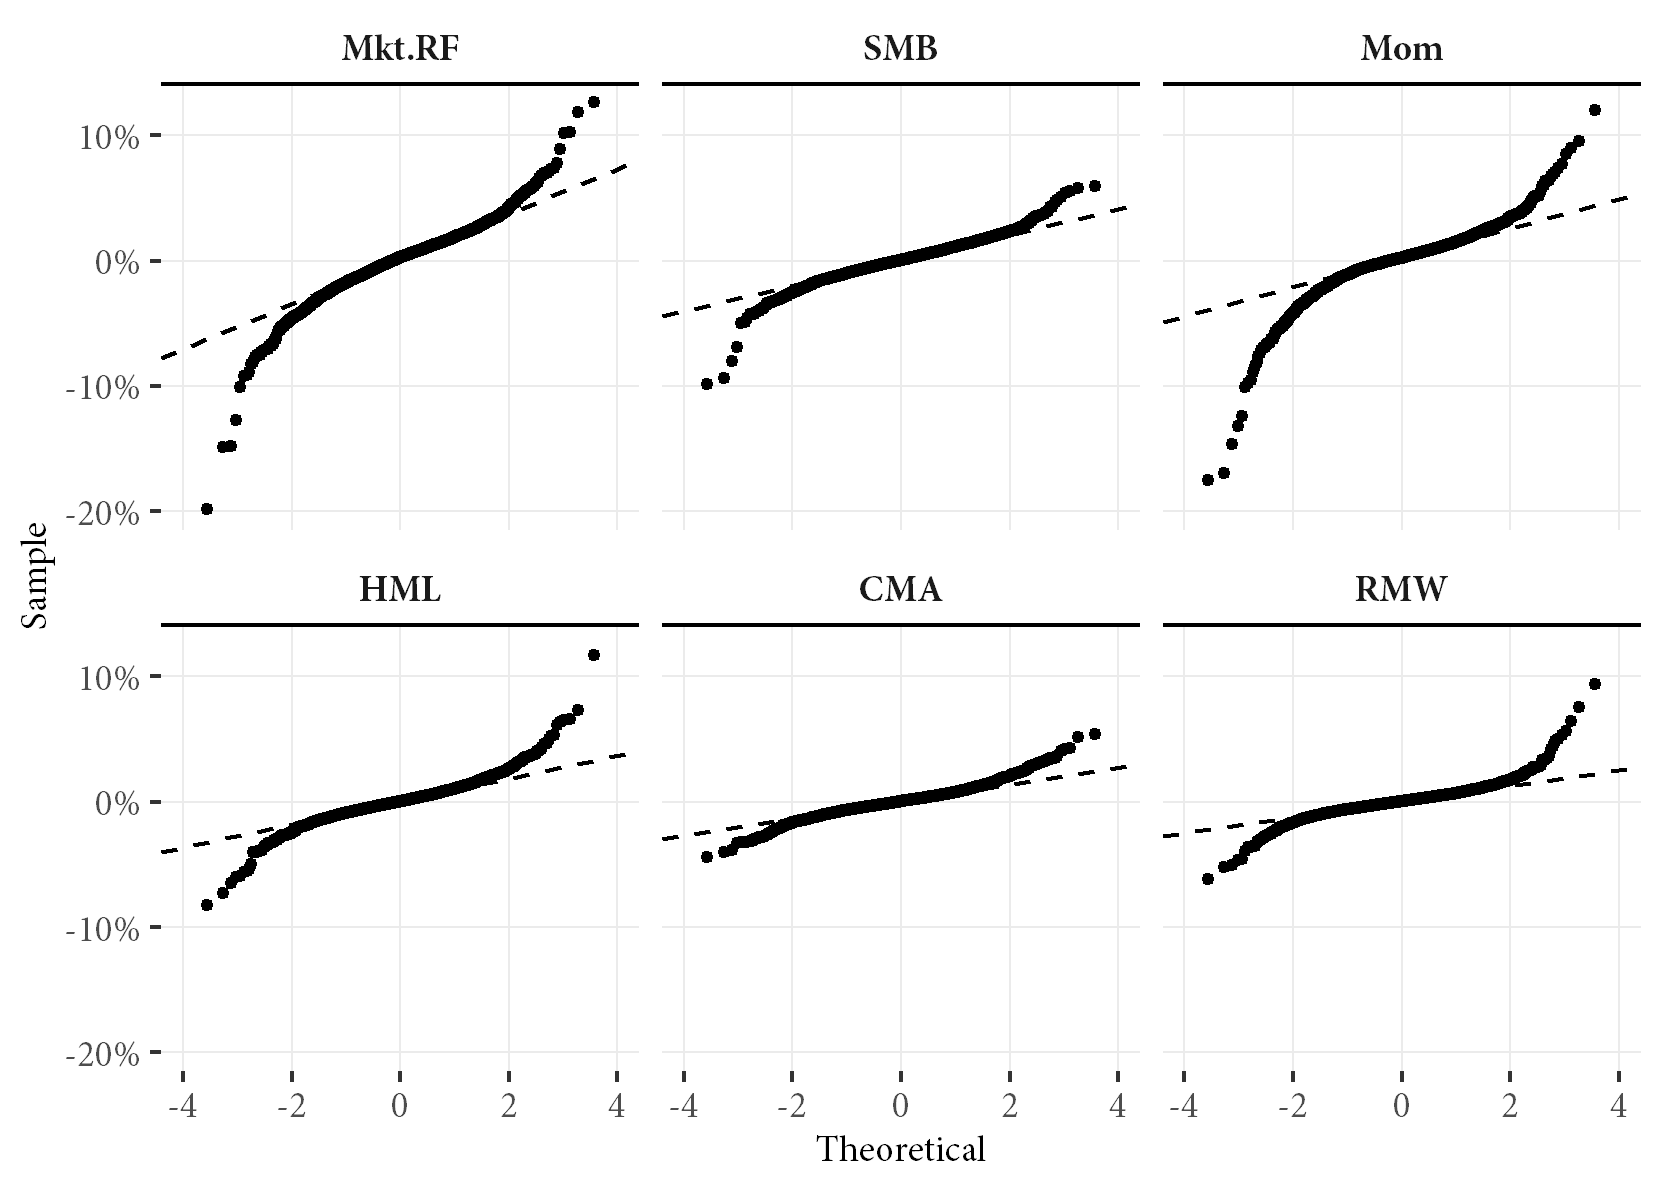
\includegraphics[scale=1]{graphics/qq_returns.png}
\end{figure}

We conduct Ljung-Box tests of the factor returns to control for weekly autocorrelation.\footnote{For a detailed description of the test, see \autoref{app:univariate_diagnostics}} The p-values of these tests are given in \autoref{tab:summarydata} and are very low for all factors except Mkt-RF, leading to a strong rejection of the zero autocorrelation null hypothesis. For Mkt-RF, the p-value is not enough for a rejection of zero autocorrelation at the 5 week maximum lag length, but strongly rejected for 10 weeks of maximum lags. We also conduct Ljung-Box tests of the squared factor returns to control for volatility clustering (ARCH effects). Here, the null hypothesis is that there are no ARCH effects, and p-values given in \autoref{tab:summarydata} strongly rejects the null for all factors at both max lag length of 5 and 10.

We conclude that factor return series are non-normal and exhibit both autocorrelation as well as autoregressive heteroscedasticity. These predictable phenomena in financial return data are typically captured by models that incorporate autoregressive components for both the conditional mean and variance equations, such as the family of ARMA-GARCH models, which are further discussed in \autoref{sec:modeling_of_factor_returns}.
\begin{figure}[htbp]
  \centering
  \footnotesize
  \renewcommand{\arraystretch}{1.2}
  \caption{Cumulative returns to factor strategies \\ \quad \\ 
  Cumulative returns to investing one dollar in each factor strategy, beginning 1963-07-05. Based on weekly returns 1963--2010.}
  \label{fig:cumret}
  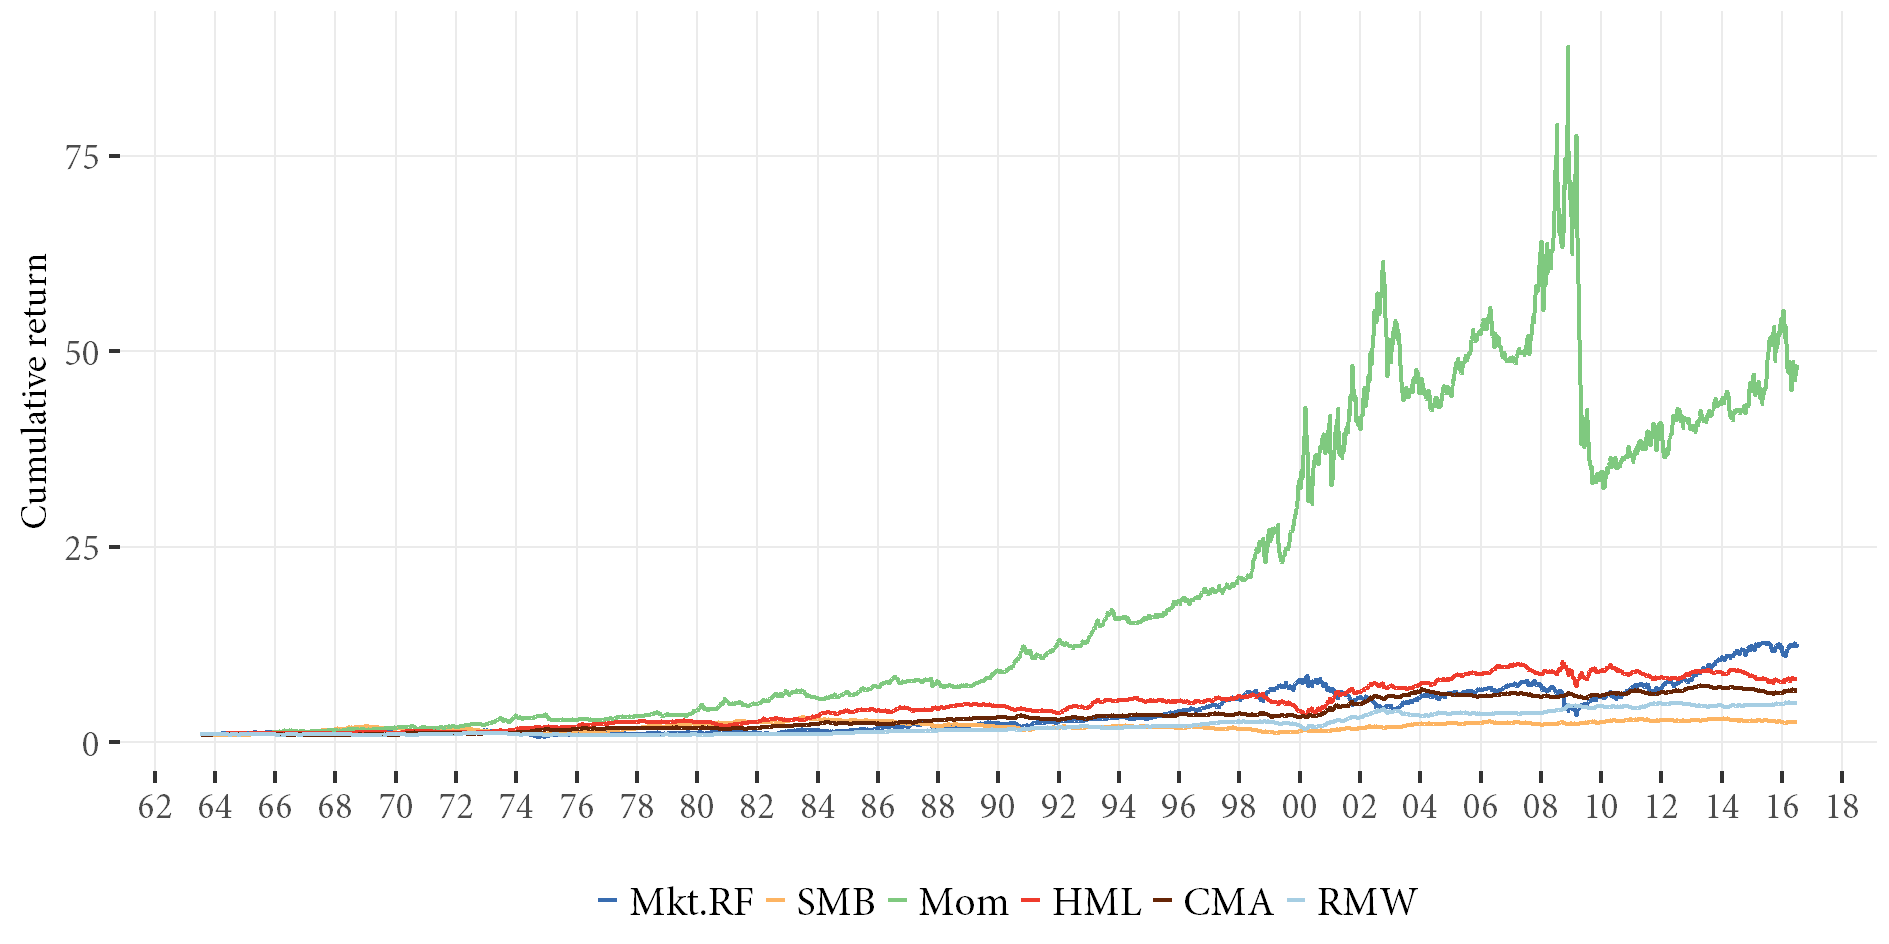
\includegraphics[scale=1]{graphics/cumretPlot.png}  
\end{figure}
\begin{figure}[htbp]
  \centering
  \footnotesize
  \renewcommand{\arraystretch}{1.2}
  \caption{Standardized cumulative returns to factor strategies \\ \quad \\ 
  Cumulative returns to investing one dollar in each factor strategy, beginning 1963-07-05. Standardized to 10\% annual volatility. Based on weekly returns 1963--2010.}
  \label{fig:cumretstd}
  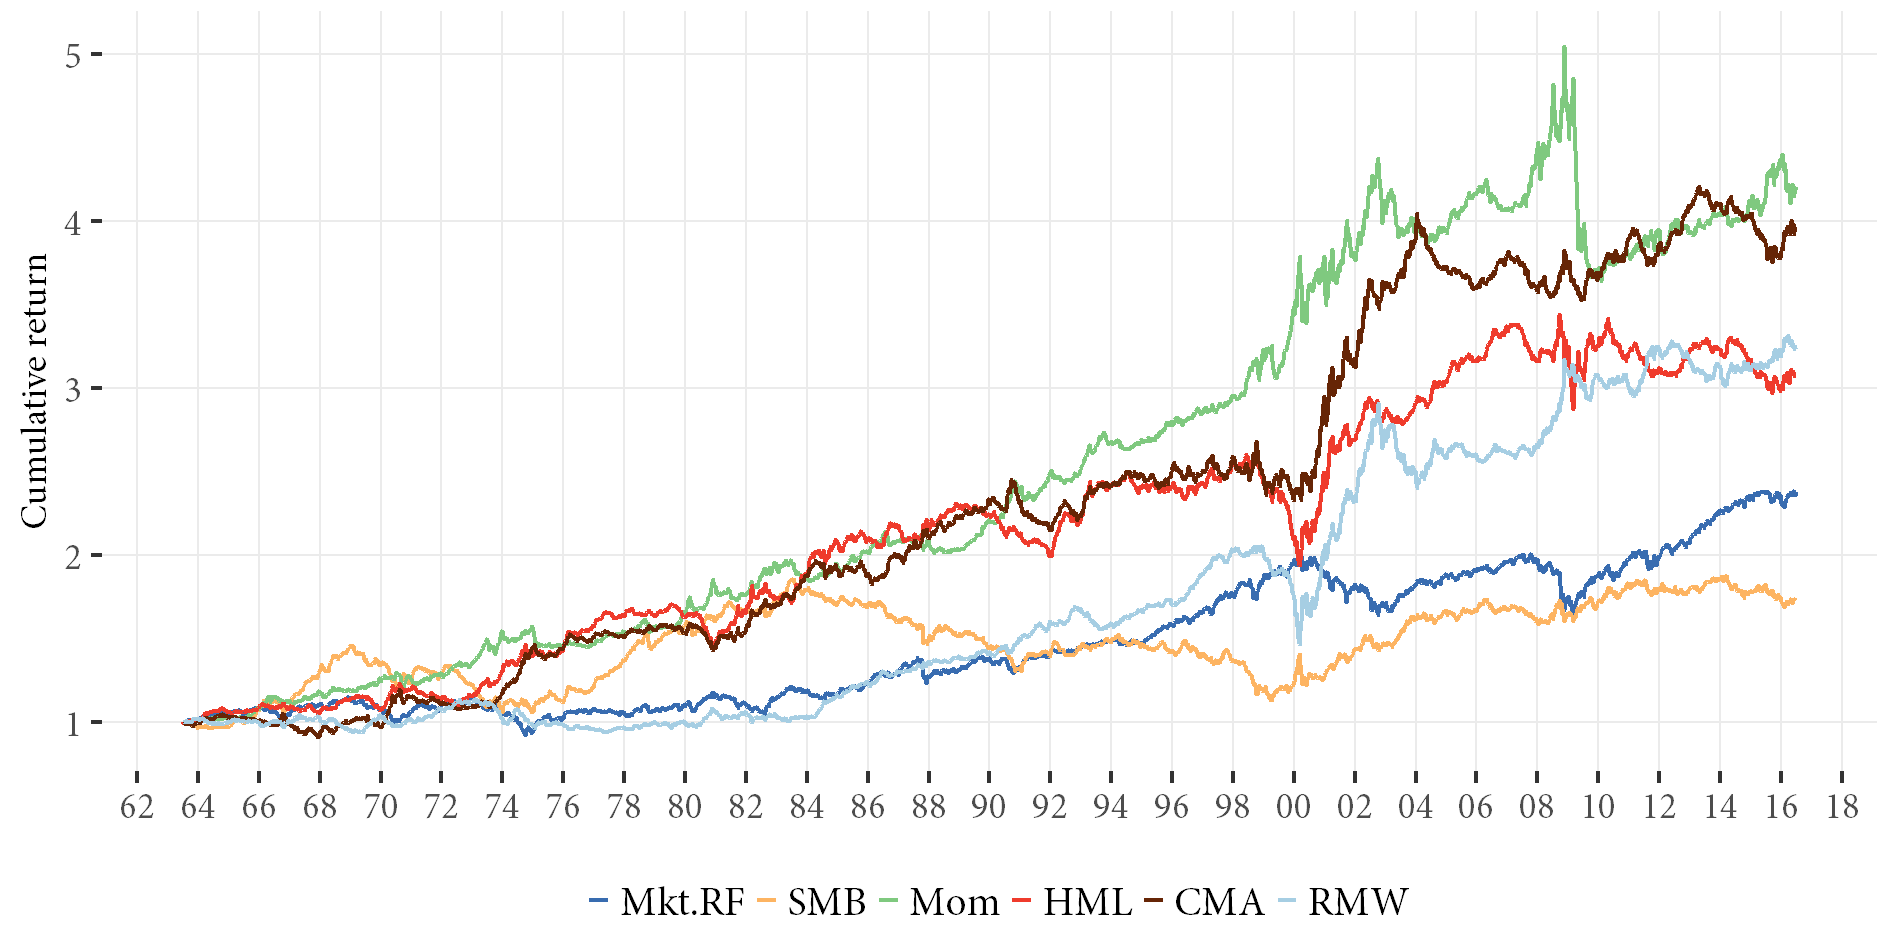
\includegraphics[scale=1]{graphics/cumretStdPlot.png}  
\end{figure}

Plots of cumulative returns (\autoref{fig:cumret}) clearly show the high returns to the momentum strategy throughout the sample period. However, normalizing the series to 10\% annual volatility (\autoref{fig:cumretstd}) gives a more nuanced picture of mean-variance performance. Since 1963, each of the strategies except for SMB has outperformed the market factor. Furthermore, factor strategies seem to crash at different times and diversify eachother, e.g. Mom performing well during 1999-2000 and RMW performing well during 2008-2009. The unconditional correlation matrix of returns is given in \autoref{tab:corr_matrix} and the general low or even negative correlation coefficients show the diversification benefits of factor strategies. The HML - CMA pair does stand out, however, with an unconditional correlation of 0.625, which could be related to a partial overlap of the factor components as discussed in \autoref{sec:literature} -- past investment is shown to be positively empirically related to the current book-to-market ratio. The substantially higher correlation in this asset pair indicates smaller diversification benefits.

\begin{table}[!htbpp] 
  \centering
  \footnotesize
  \renewcommand{\arraystretch}{1.2}
  \caption{Correlation matrix \\ \quad \\
  Unconditional sample correlation matrix of factor return series. Based on weekly return data 1963--2016}
  \label{tab:corr_matrix} 
\begin{tabularx}{\textwidth}{@{\extracolsep{5pt}} X D{.}{.}{1} D{.}{.}{1} D{.}{.}{1} D{.}{.}{1} D{.}{.}{1} D{.}{.}{1}} 
  \toprule
  & \multicolumn{1}{c}{Mkt-RF} & \multicolumn{1}{c}{SMB} & \multicolumn{1}{c}{Mom} & \multicolumn{1}{c}{HML} & \multicolumn{1}{c}{CMA} & \multicolumn{1}{c}{RMW} \\ 
\midrule
\text{Mkt.RF} & $1.000$ & $$ & $$ & $$ & $$ & $$ \\ 
\text{SMB} & $0.086$ & $1.000$ & $$ & $$ & $$ & $$ \\ 
\text{Mom} & $$-$0.113$ & $$-$0.007$ & $1.000$ & $$ & $$ & $$ \\ 
\text{HML} & $$-$0.283$ & $$-$0.026$ & $$-$0.219$ & $1.000$ & $$ & $$ \\ 
\text{CMA} & $$-$0.416$ & $$-$0.048$ & $0.071$ & $0.625$ & $1.000$ & $$ \\ 
\text{RMW} & $$-$0.154$ & $$-$0.337$ & $0.080$ & $$-$0.054$ & $$-$0.067$ & $1.000$ \\ 
\bottomrule
\end{tabularx} 
\end{table}
